\chapter{Rotations, Quaternions and Rigid-Body Kinematics}
\label{ch:rotations}
\chaptermark{Rotations and Quaternions} % short running header

\begin{objectives}
\begin{itemize}
  \item Read and write frame-annotated transformations such as $R_{wb}$, $p_{wb}$ and $T_{bc}$ without ambiguity, and catch frame bugs
        with the adjacency rule.
  \item Understand rotations in the plane, then in space: rotation matrices, axis-angle and Rodrigues' formula.
  \item Understand Euler angles, intrinsic versus extrinsic sequences, their conversions, and why they are banned from the estimator.
  \item Derive Hamilton quaternion algebra and its rotation formula; convert between quaternions and matrices; interpolate; and
        translate formulas from the JPL convention.
  \item Derive the kinematics of rotating bodies: $\dot R = R\sx{\omega}$, $\dot q = \tfrac12 q\qprod[0,\omega]$, the transport theorem and the Coriolis
        acceleration, and quantify the effects of the Earth's rotation.
\end{itemize}
\end{objectives}

% ==============================================================================
\section{Frames and notation}

A \term{frame} is an origin together with three orthonormal, right-handed axes. Three frames appear in this project (\cref{fig:frames}).

\begin{convention}[frames, AGENTS.md C1]
\begin{itemize}
  \item $W$, the \textbf{world} frame: fixed, gravity-aligned with $z$ pointing up, the frame of the ground truth (EuRoC calls it
        \code{R}). Gravity is $g_w = [0, 0, -9.81]\T~\mathrm{m/s^2}$.
  \item $B$, the \textbf{body} frame: the IMU frame \code{imu0} (EuRoC's \code{S} in \code{imu0}).
  \item $C$, the left \textbf{camera} frame \code{cam0}: origin at the optical center, $z$ along the optical axis, $x$ to the right and $y$
        down in the image.
\end{itemize}
$R_{wb}$ (or $q_{wb}$) maps body-frame coordinates to world-frame coordinates, $v_w = R_{wb}v_b$. $p_{wb}$ is the position of the origin of $B$
expressed in $W$. $v_{wb}$ is the velocity of $B$ relative to $W$, expressed in $W$. $T_{bc} = (R_{bc}, p_{bc})$ maps camera points into the body
frame, $p_b = R_{bc}p_c + p_{bc}$; it is \code{T\_BS} from \code{cam0/sensor.yaml}. A world-to-body rotation is never used as a state.
\end{convention}

\begin{figure}[t]
\centering
\begin{tikzpicture}[scale=1.0]
  \coordinate (W) at (0,0);
  \draw[frameaxis, plotorange] (W) -- ++(1.4,0) node[right] {$x_w$};
  \draw[frameaxis, plotgreen] (W) -- ++(0.75,0.6) node[above right] {$y_w$};
  \draw[frameaxis, plotblue] (W) -- ++(0,1.4) node[above] {$z_w$};
  \node[below left] at (W) {$W$};
  \draw[->, thick, black!60] (-0.6,1.0) -- ++(0,-0.8) node[midway, left] {$g$};
  \coordinate (B) at (5.2,2.2);
  \begin{scope}[shift={(B)}, rotate=25]
    \draw[fill=primarylight, draw=primary, rounded corners=2pt] (-0.55,-0.25) rectangle (0.55,0.25);
    \draw[frameaxis, plotorange] (0,0) -- (1.3,0) node[right] {$x_b$};
    \draw[frameaxis, plotgreen] (0,0) -- (0.65,0.55) node[above right] {$y_b$};
    \draw[frameaxis, plotblue] (0,0) -- (0,1.3) node[above] {$z_b$};
    \node[below left] at (-0.2,-0.25) {$B$ (IMU)};
    \coordinate (C) at (2.0,-1.3);
    \draw[fill=white, draw=primary] ($(C)+(-0.15,0.15)$) rectangle ($(C)+(0.15,-0.15)$);
    \draw[frameaxis, plotblue] (C) -- ++(0,-0.9) node[below] {$z_c$};
    \draw[frameaxis, plotorange] (C) -- ++(0.8,0) node[right] {$x_c$};
    \draw[frameaxis, plotgreen] (C) -- ++(-0.45,-0.35) node[left] {$y_c$};
    \node[above right] at ($(C)+(0.1,0.1)$) {$C$};
    \draw[->, thick, conv] (0.3,-0.3) to[bend right=20] node[midway, below left=-1pt] {$T_{bc}$} ($(C)+(-0.2,0.05)$);
  \end{scope}
  \draw[->, thick, primary, dashed] (W) -- (B) node[midway, above left] {$p_{wb}$, $R_{wb}$};
\end{tikzpicture}
\caption{The world frame $W$ (gravity-aligned, $z$ up), the body/IMU frame $B$ moving with the vehicle, and the camera frame $C$ rigidly
attached to the body through the constant extrinsic calibration $T_{bc}$.}
\label{fig:frames}
\end{figure}

\subsection{Reading subscripts}

The naming rule \code{<quantity>\_<to><from>} makes products self-checking. $R_{wb}$ takes a vector \emph{from} $B$ \emph{to} $W$. Composition
chains frames like dominoes:
\begin{equation}
  R_{wc} = R_{wb}\,R_{bc}, \qquad v_w = R_{wb}\,R_{bc}\,v_c .
\end{equation}

\begin{keyidea}[the adjacency rule]
\index{adjacency rule}
In a valid product, adjacent subscripts match: $R_{w\underline{b}}\,R_{\underline{b}c}$. A product such as $R_{wb}R_{cb}$ has mismatched neighbors and is
a bug. The fix is a transpose, $R_{wb}R_{cb}\T = R_{wb}R_{bc}$, since $R_{bc} = R_{cb}\inv = R_{cb}\T$. Apply the rule to every line of code that
multiplies rotations or transforms points.
\end{keyidea}

\subsection{Active and passive views}

A rotation matrix can be read in two ways. In the \emph{passive} view, $R_{wb}$ re-expresses the same physical vector in another frame:
$v_w$ and $v_b$ are coordinates of one arrow (\cref{sec:orthogonal-matrices}). In the \emph{active} view, $R_{wb}$ rotates the world axes
onto the body axes: its columns are the body axes $x_b, y_b, z_b$ expressed in world coordinates. Both readings describe the same matrix:
\begin{equation}
  R_{wb} = \begin{bmatrix} x_b^{(w)} & y_b^{(w)} & z_b^{(w)} \end{bmatrix}.
\end{equation}
This gives a quick sanity check when debugging: the third column of $R_{wb}$ is the body $z$-axis in world coordinates. For a level
vehicle whose $z$-axis points up, it is $[0,0,1]\T$; its third row is the world vertical expressed in the body frame.

% ==============================================================================
\section{Rotations in the plane}

Planar rotations contain most of the ideas of this chapter in their simplest form. The rotation by $\theta$ is (\cref{ex:rot2d})
\begin{equation}
  R(\theta) = \begin{bmatrix} \cos\theta & -\sin\theta \\ \sin\theta & \cos\theta \end{bmatrix}.
\end{equation}
Rotations compose by adding angles, $R(\alpha)R(\beta) = R(\alpha + \beta)$ (multiply out and use the angle-addition formulas), so planar
rotations commute. The angle is a perfect coordinate: $R(\theta)$ is determined by $\theta$, and every planar rotation is $R(\theta)$ for a
$\theta$ that is unique up to multiples of $2\pi$. The only subtlety is wrap-around: angles must be compared modulo $2\pi$, which is why the
difference between two headings is computed as $\atantwo(\sin(\theta_2 - \theta_1), \cos(\theta_2 - \theta_1))$ rather than $\theta_2 - \theta_1$.

Identifying the plane with the complex numbers, rotation by $\theta$ is multiplication by $e^{i\theta} = \cos\theta + i\sin\theta$. Unit complex
numbers compose by multiplication, and their angles add. Quaternions (\cref{sec:quaternions}) are the three-dimensional generalization of
this idea, with one crucial difference: in three dimensions, rotations do not commute.

% ==============================================================================
\section{Rotation matrices and \texorpdfstring{$\SO$}{SO(3)}}

\begin{definition}[Special orthogonal group]
\index{special orthogonal group}
$\SO = \{ R \in \R^{3\times3} : R\T R = I,\ \det R = +1 \}$.
\end{definition}

Orthogonality ($R\T R = I$) means $R$ preserves lengths and angles; $\det R = +1$ excludes reflections, which would turn a right-handed
frame into a left-handed one (\cref{sec:orthogonal-matrices}). The set is closed under multiplication and inversion, $R\inv = R\T$, so it is
a \emph{group}. A rotation matrix has nine entries but only three degrees of freedom: orthonormality imposes six constraints (three unit
lengths, three orthogonalities). This redundancy is why $\SO$ is a curved three-dimensional surface inside the nine-dimensional space of
matrices rather than a vector space; the sum of two rotation matrices is not a rotation matrix.

The elementary rotations about the coordinate axes follow from the planar case:
\begin{equation}
  R_x(\alpha) = \begin{bmatrix} 1 & 0 & 0 \\ 0 & c_\alpha & -s_\alpha \\ 0 & s_\alpha & c_\alpha \end{bmatrix},\quad
  R_y(\alpha) = \begin{bmatrix} c_\alpha & 0 & s_\alpha \\ 0 & 1 & 0 \\ -s_\alpha & 0 & c_\alpha \end{bmatrix},\quad
  R_z(\alpha) = \begin{bmatrix} c_\alpha & -s_\alpha & 0 \\ s_\alpha & c_\alpha & 0 \\ 0 & 0 & 1 \end{bmatrix},
\end{equation}
with $c_\alpha = \cos\alpha$, $s_\alpha = \sin\alpha$. (The signs of $R_y$ look reversed but are not: in the $z$-$x$ plane, ordered cyclically
after $y$, it is the usual planar rotation.) Rotations in space do not commute: $R_x(90^\circ)R_y(90^\circ) \ne R_y(90^\circ)R_x(90^\circ)$. Try it
with a book.

\section{Axis-angle and Rodrigues' formula}

By Euler's theorem (\cref{thm:euler-axis}), every rotation is a rotation by some angle $\theta \in [0, \pi]$ about some unit axis $u$. The pair
$(u, \theta)$ is the \term{axis-angle} representation, and $\phi = \theta u \in \R^3$ is the \term{rotation vector}: its direction is the axis and its
length the angle. The rotation vector is the central object of \cref{ch:lie}.

\begin{theorem}[Rodrigues' rotation formula]
\label{thm:rodrigues}
\index{Rodrigues' formula}
The rotation by angle $\theta$ about the unit axis $u$ is
\begin{equation}
  R = I + \sin\theta\,\sx{u} + (1 - \cos\theta)\,\sx{u}^2
    = \cos\theta\, I + (1-\cos\theta)\,u u\T + \sin\theta\,\sx{u}.
  \label{eq:rodrigues}
\end{equation}
\end{theorem}
\begin{proof}[Geometric proof]
Split any vector into components parallel and perpendicular to the axis (\cref{prop:projection-line}), $v = v_\parallel + v_\perp$ with
$v_\parallel = u u\T v$. Rotation leaves $v_\parallel$ unchanged and rotates $v_\perp$ by $\theta$ within the plane spanned by $v_\perp$ and
$u \times v_\perp = u \times v$ (a vector of the same length, rotated $90^\circ$ about $u$):
\begin{equation*}
  Rv = v_\parallel + \cos\theta\, v_\perp + \sin\theta\, u \times v .
\end{equation*}
Substituting $v_\perp = v - uu\T v = -\sx{u}^2 v$ (from \eqref{eq:skew-sq} with $\|u\|=1$) and $u \times v = \sx{u}v$ gives
$Rv = (I + \sin\theta\sx{u} + (1 - \cos\theta)\sx{u}^2)v$.
\end{proof}
\begin{proof}[Algebraic proof]
The rotation about $u$ at unit angular rate satisfies $\dot R = \sx{u} R$ (\cref{sec:rot-kinematics}), so $R(\theta) = \exp(\theta\sx{u})$ by
\cref{thm:lti-solution}. With $\sx{u}^3 = -\sx{u}$ from \eqref{eq:skew-cube}, all odd powers of $\sx{u}$ are $\pm\sx{u}$ and all even powers
(except the zeroth) are $\pm\sx{u}^2$, so the exponential series regroups as
\begin{equation*}
  \exp(\theta\sx{u}) = I + \Big(\theta - \tfrac{\theta^3}{3!} + \tfrac{\theta^5}{5!} - \cdots\Big)\sx{u}
     + \Big(\tfrac{\theta^2}{2!} - \tfrac{\theta^4}{4!} + \cdots\Big)\sx{u}^2,
\end{equation*}
and the two series are $\sin\theta$ and $1 - \cos\theta$.
\end{proof}

Two consequences of \eqref{eq:rodrigues} recover $(u, \theta)$ from $R$. Taking the trace (using $\tr\sx{u} = 0$ and $\tr\sx{u}^2 = -2$) and the
skew-symmetric part,
\begin{equation}
  \tr R = 1 + 2\cos\theta, \qquad R - R\T = 2\sin\theta\,\sx{u}.
  \label{eq:trace-angle}
\end{equation}
\Cref{ch:lie} shows that \emph{how} these are combined numerically matters a great deal.

\begin{worked}[a quarter turn]
Rotate by $\theta = 90^\circ$ about $u = e_z$: $\sx{e_z} = \begin{bmatrix}0 & -1 & 0\\1 & 0 & 0\\0 & 0 & 0\end{bmatrix}$ and
$\sx{e_z}^2 = \diag(-1, -1, 0)$, so \eqref{eq:rodrigues} gives $R = \begin{bmatrix}0 & -1 & 0\\ 1 & 0 & 0\\ 0 & 0 & 1\end{bmatrix} = R_z(90^\circ)$, which
sends $e_x$ to $e_y$, as a counter-clockwise quarter turn about $z$ should. Its trace is $1 = 1 + 2\cos90^\circ$.
\end{worked}

% ==============================================================================
\section{Euler angles}

\subsection{Definition and the two readings}

\term{Euler angles} describe a rotation as three successive rotations about coordinate axes. The aerospace yaw-pitch-roll ($ZYX$)
convention writes
\begin{equation}
  R_{wb} = R_z(\psi)\,R_y(\vartheta)\,R_x(\varphi),
  \label{eq:zyx}
\end{equation}
with yaw $\psi$, pitch $\vartheta$ and roll $\varphi$. The same product can be read in two ways, which are a constant source of confusion:
\begin{itemize}
  \item \emph{Intrinsic} (rotating axes): start aligned with the world, yaw by $\psi$ about $z$, then pitch by $\vartheta$ about the \emph{new} $y$-axis,
        then roll by $\varphi$ about the \emph{newest} $x$-axis. This is how a pilot thinks.
  \item \emph{Extrinsic} (fixed axes): roll by $\varphi$ about the world $x$-axis, then pitch by $\vartheta$ about the world $y$-axis, then yaw by $\psi$ about
        the world $z$-axis.
\end{itemize}
Both readings produce the same matrix \eqref{eq:zyx}; the intrinsic sequence $z, y', x''$ equals the extrinsic sequence $x, y, z$ in reverse
order. Twelve different axis sequences are in use, and each library documents its own. Always check the convention against a known example
before trusting a conversion.

\subsection{Conversions}

Multiplying out \eqref{eq:zyx} gives the third row of $R$ as $(-\sin\vartheta,\ \cos\vartheta\sin\varphi,\ \cos\vartheta\cos\varphi)$ and the first column as
$\cos\vartheta(\cos\psi, \sin\psi, \cdot)$. Hence
\begin{equation}
  \vartheta = \atantwo\big(-R_{31},\ \sqrt{R_{11}^2 + R_{21}^2}\big), \qquad
  \varphi = \atantwo(R_{32},\ R_{33}), \qquad
  \psi = \atantwo(R_{21},\ R_{11}) .
\end{equation}
When $\cos\vartheta = 0$ ($\vartheta = \pm90^\circ$), the formulas for $\varphi$ and $\psi$ become $\atantwo(0, 0)$: only their sum or difference is determined.

\subsection{Gimbal lock}

The relation between the body angular velocity measured by a gyroscope and the rates of the Euler angles is
\begin{equation}
  \begin{bmatrix} \dot\varphi \\ \dot\vartheta \\ \dot\psi \end{bmatrix}
  = \begin{bmatrix}
      1 & \sin\varphi\tan\vartheta & \cos\varphi\tan\vartheta \\
      0 & \cos\varphi & -\sin\varphi \\
      0 & \sin\varphi/\cos\vartheta & \cos\varphi/\cos\vartheta
    \end{bmatrix} \omega_b ,
  \label{eq:euler-rates}
\end{equation}
obtained by differentiating \eqref{eq:zyx} and comparing with $\sx{\omega_b} = R\T\dot R$ (\cref{sec:rot-kinematics}). At $\vartheta = \pm90^\circ$ the
matrix blows up. Geometrically, when the nose points straight up, yaw and roll rotate about the same physical axis, so the three angles no
longer describe three independent motions. This is \term{gimbal lock}, named after mechanical gimbal platforms that physically jam in this
configuration. Near the singularity, small angular velocities produce enormous Euler-angle rates, and a filter that linearizes in Euler
angles becomes numerically meaningless.

\begin{convention}[AGENTS.md C2]
Euler angles never appear in the estimator. They may appear only in telemetry and plots.
\end{convention}

No three-parameter representation of $\SO$ is free of singularities everywhere: a topological fact (the space $\SO$ cannot be covered by a
single chart). The solution adopted by modern estimators is to store attitude in a singularity-free \emph{redundant} representation (a unit
quaternion or a rotation matrix) and to use three parameters only for \emph{small} deviations around the current estimate, where no
singularity is near. That is the content of \cref{ch:lie}.

% ==============================================================================
\section{Quaternions}
\label{sec:quaternions}

\subsection{Quaternion algebra}

\index{quaternion}
A \term{quaternion} is a four-component number $q = w + x\,i + y\,j + z\,k$, written as a scalar part and a vector part, $q = [w,\ v]$ with
$v = (x,y,z)\T$. Hamilton's multiplication rules for the three imaginary units are
\begin{equation}
  i^2 = j^2 = k^2 = ijk = -1,
\end{equation}
from which $ij = k = -ji$, $jk = i = -kj$ and $ki = j = -ik$. (For example, multiplying $ijk = -1$ on the right by $k$ gives $ij(-1) = -k$.)
Expanding the product of two quaternions term by term with these rules and collecting the scalar and vector parts gives
\begin{equation}
  p \qprod q = \begin{bmatrix} p_w q_w - p_v\T q_v \\ p_w q_v + q_w p_v + p_v \times q_v \end{bmatrix}.
  \label{eq:qprod}
\end{equation}
The products of imaginary units produce exactly the components of the cross product, which makes the product non-commutative:
$p\qprod q - q\qprod p = [0,\ 2p_v\times q_v]$. It is associative. Because it is linear in each factor, it can be written with matrices,
\begin{equation}
  p\qprod q = [p]_L\, q = [q]_R\, p, \qquad
  [p]_L = \begin{bmatrix} p_w & -p_v\T \\ p_v & p_w I + \sx{p_v} \end{bmatrix}, \quad
  [q]_R = \begin{bmatrix} q_w & -q_v\T \\ q_v & q_w I - \sx{q_v} \end{bmatrix},
\end{equation}
where quaternions are treated as 4-vectors $[q_w;\ q_v]$.

The \emph{conjugate} is $q^* = [w,\ -v]$ and the \emph{norm} is $\|q\| = \sqrt{w^2 + \|v\|^2}$. By \eqref{eq:qprod}, $q\qprod q^* = [\|q\|^2,\ 0]$, so the
inverse is $q\inv = q^*/\|q\|^2$. Conjugation reverses products, $(p\qprod q)^* = q^*\qprod p^*$, and norms multiply, $\|p\qprod q\| = \|p\|\|q\|$
(because $\|p\qprod q\|^2 = p\qprod q\qprod q^*\qprod p^* = \|q\|^2\,p\qprod p^* = \|p\|^2\|q\|^2$). Consequently the product of two \emph{unit}
quaternions is a unit quaternion: unit quaternions form a group, the three-dimensional sphere $S^3 \subset \R^4$.

\subsection{Unit quaternions represent rotations}

Identify a vector $a \in \R^3$ with the \emph{pure} quaternion $[0, a]$.

\begin{theorem}[Rotation by a unit quaternion]
\label{thm:quat-rotation}
For a unit quaternion $q = [w, v]$, the map $a \mapsto q\qprod[0, a]\qprod q^*$ sends pure quaternions to pure quaternions and acts on $a$ as the rotation
matrix
\begin{equation}
  R(q) = (w^2 - v\T v)\,I + 2\,v v\T + 2w\,\sx{v}
  = \begin{bmatrix}
    1 - 2(y^2 + z^2) & 2(xy - wz) & 2(xz + wy) \\
    2(xy + wz) & 1 - 2(x^2 + z^2) & 2(yz - wx) \\
    2(xz - wy) & 2(yz + wx) & 1 - 2(x^2 + y^2)
  \end{bmatrix}.
  \label{eq:quat-to-rot}
\end{equation}
The unit quaternion of a rotation by $\theta$ about the unit axis $u$ is
\begin{equation}
  q = \big[\cos(\theta/2),\ \sin(\theta/2)\,u\big].
  \label{eq:quat-axis-angle}
\end{equation}
\end{theorem}
\begin{proof}
By \eqref{eq:qprod}, $[0, a]\qprod q^* = [a\T v,\ wa - a\times v]$. Multiplying on the left by $q = [w, v]$:
the scalar part is $w\,a\T v - v\T(wa - a\times v) = 0$ (since $v\T(a\times v) = 0$), and the vector part is
$w(wa - a\times v) + (a\T v)v + v\times(wa - a\times v) = w^2a + 2w\,v\times a + (v\T a)v - v\times(a\times v)$. With the BAC--CAB rule,
$v\times(a\times v) = a\,(v\T v) - v\,(v\T a)$, so the vector part is $(w^2 - v\T v)a + 2(v\T a)v + 2w\,v\times a$, which is \eqref{eq:quat-to-rot}. This
matrix is orthogonal with determinant one (it preserves norms, because quaternion norms multiply, and depends continuously on $q$, equal to
$I$ at $q = [1, 0]$). For \eqref{eq:quat-axis-angle}, substitute $w = \cos\frac\theta2$, $v = \sin\frac\theta2 u$ and use the double-angle identities
$w^2 - v\T v = \cos\theta$, $2\sin^2\frac\theta2 = 1 - \cos\theta$ and $2\sin\frac\theta2\cos\frac\theta2 = \sin\theta$; the result is the second form of
Rodrigues' formula \eqref{eq:rodrigues}.
\end{proof}

The \emph{half} angle in \eqref{eq:quat-axis-angle} is the most common source of factor-of-two bugs. It arises because $q$ appears twice in the
sandwich product $q \qprod [0,a] \qprod q^*$, each occurrence contributing half of the rotation.

\begin{keyidea}[double cover]
\index{double cover}
$q$ and $-q$ give the same $R(q)$, since \eqref{eq:quat-to-rot} is quadratic in $q$. Every rotation has exactly two unit quaternions, at opposite
points of the sphere $S^3$. They correspond to rotating by $\theta$ about $u$, or by $2\pi - \theta$ about $-u$. Code that compares, averages,
interpolates or takes logarithms of quaternions must account for this. The project canonicalizes to $w \ge 0$ before taking $\Log_q$
(AGENTS.md C2).
\end{keyidea}

\subsection{Composition}

Because $(p\qprod q)\qprod[0, a]\qprod(p\qprod q)^* = p\qprod\big(q\qprod[0, a]\qprod q^*\big)\qprod p^*$, the Hamilton product composes rotations in the same order
as matrix multiplication:
\begin{equation}
  R(p \qprod q) = R(p)\,R(q), \qquad q_{wc} = q_{wb}\qprod q_{bc} \ \leftrightarrow\ R_{wc} = R_{wb}R_{bc}.
\end{equation}
The adjacency rule therefore applies to quaternions unchanged. Composing quaternions costs 16 multiplications and 12 additions, against 27 and
18 for matrices, and renormalizing a quaternion is trivial compared with re-orthogonalizing a matrix. These are the practical reasons to
store attitude as a quaternion.

\begin{worked}[composing two quarter turns]
The quarter turn about $z$ is $q_z = [\cos45^\circ,\ \sin45^\circ e_z] = \frac{1}{\sqrt2}[1, (0,0,1)]$, and about $x$ it is
$q_x = \frac{1}{\sqrt2}[1, (1,0,0)]$. By \eqref{eq:qprod}, $q_z\qprod q_x = \tfrac12\big[1,\ (1, 0, 1) + e_z\times e_x\big] = \tfrac12[1, (1, 1, 1)]$: a rotation by
$2\arccos\frac12 = 120^\circ$ about $(1,1,1)/\sqrt3$. (Check: it cycles the axes, $x\to y\to z\to x$.) In the other order,
$q_x\qprod q_z = \tfrac12[1, (1, -1, 1)]$, a different rotation.
\end{worked}

\subsection{Converting a rotation matrix to a quaternion}

Inverting \eqref{eq:quat-to-rot} naively via $w = \tfrac12\sqrt{1 + \tr R}$ and $v = (R - R\T)\veeop/(4w)$ divides by a number that vanishes for
$180^\circ$ rotations. \emph{Shepperd's method} avoids this. From \eqref{eq:quat-to-rot}, the four quantities
$4w^2 = 1 + \tr R$, $4x^2 = 1 + R_{11} - R_{22} - R_{33}$, $4y^2 = 1 - R_{11} + R_{22} - R_{33}$ and $4z^2 = 1 - R_{11} - R_{22} + R_{33}$ can all be computed
from the diagonal. Choose the largest (at least $1/4$, since $w^2 + x^2 + y^2 + z^2 = 1$), take its square root, and compute the other three components
from the off-diagonal sums and differences, for example $4wx = R_{32} - R_{23}$, $4xy = R_{21} + R_{12}$, $4xz = R_{13} + R_{31}$, dividing only by the large
component. Eigen implements this method.

\subsection{The Hamilton and JPL conventions}

Unfortunately, two incompatible quaternion conventions are in wide use. Much of the classic VIO literature, including the original MSCKF
paper~\cite{mourikis2007msckf} and the indirect Kalman filter report of Trawny and Roumeliotis~\cite{trawny2005indirect}, uses the
\emph{JPL} convention. Formulas cannot be copied between the two without translation~\cite{sommer2018flipped}.

\begin{table}[h]
\centering\small
\begin{tabularx}{\textwidth}{@{}l X X@{}}
\toprule
 & \textbf{Hamilton (this project)} & \textbf{JPL} \\
\midrule
Multiplication rule & $ij = k$ ($ijk = -1$) & $ij = -k$ ($ijk = +1$) \\
Component order & usually $[w, x, y, z]$ & usually $[x, y, z, w]$ \\
Typical meaning & body-to-world (active), $q_{wb}$ & world-to-body (passive), ${}^{B}_{W}\bar q$ \\
Composition & $q_{wc} = q_{wb}\qprod q_{bc}$ & ${}^{C}_{W}\bar q = {}^{C}_{B}\bar q\otimes{}^{B}_{W}\bar q$ \\
Rotation matrix & $R(q) = (w^2 - v\T v)I + 2vv\T + 2w\sx{v}$ & $C(\bar q) = (2q_4^2 - 1)I - 2q_4\sx{q} + 2qq\T$ \\
Used by & Eigen, ROS, Sol\`a~\cite{sola2017quaternion}, Ceres, Sophus & MSCKF papers, Trawny~\cite{trawny2005indirect}, NASA \\
\bottomrule
\end{tabularx}
\caption{Hamilton versus JPL quaternions. The JPL product of two quaternions equals the Hamilton product of the same numbers in reverse order.}
\label{tab:hamilton-jpl}
\end{table}

A useful fact for reading the JPL literature: the JPL quaternion ${}^B_W\bar q$ of the world-to-body rotation has \emph{the same four numbers} as the
Hamilton quaternion $q_{wb}$ of the body-to-world rotation, merely stored in the order $[x, y, z, w]$. (Substitute into the two rotation formulas of
\cref{tab:hamilton-jpl}: $C(\bar q) = R(q)\T$.) What changes is the meaning of products and of perturbations: a JPL error quaternion
$\delta\bar q$ in ${}^B_W\bar q = \delta\bar q\otimes{}^B_W\hat{\bar q}$ is a perturbation in the body frame, but written on the left, and its Jacobians differ in sign
and order from ours. Translate a JPL derivation by re-deriving it, not by pattern-matching symbols.

\begin{convention}[quaternions, AGENTS.md C2]
Hamilton quaternions, \code{Eigen::Quaterniond}, always of unit norm, normalized after every multiplicative update. Never substitute JPL
formulas, even when a paper you are reading uses them. Translate them first.
\end{convention}

\subsection{Quaternions in code and data}

\begin{pitfall}[coefficient order]
Three orderings meet at the project's input boundary:
\begin{itemize}
  \item \code{Eigen::Quaterniond(w, x, y, z)}: the constructor takes $w$ \emph{first};
  \item \code{q.coeffs()}: Eigen's storage is $[x, y, z, w]$, with $w$ \emph{last};
  \item EuRoC CSV files store \code{qw, qx, qy, qz}, with $w$ first.
\end{itemize}
Mapping a raw EuRoC row with \code{Eigen::Map<Quaterniond>} interprets it as $[x,y,z,w]$ and silently produces a different, valid-looking
rotation. Always construct explicitly, \code{Eigen::Quaterniond(row[0], row[1], row[2], row[3])}, and cover the parser with a fixture test.
\end{pitfall}

Other Eigen facts worth knowing: \code{q * v} for a \code{Vector3d} applies $R(q)$ to $v$; \code{q1 * q2} is the Hamilton product;
\code{q.conjugate()} is the inverse of a unit quaternion; \code{q.normalize()} works in place while \code{q.normalized()} returns a copy; and
\code{q.toRotationMatrix()} evaluates \eqref{eq:quat-to-rot}.

\paragraph{Normalization.} Each multiplicative update of a quaternion rounds its four components, so $\|q\|$ performs a slow random walk away
from $1$. A non-unit quaternion inserted into \eqref{eq:quat-to-rot} produces a matrix that scales vectors by $\|q\|^2$ as well as rotating them.
Dividing by the norm after every update costs a few flops and removes the problem. Milestone 4 checks that $|\|q\| - 1| < 10^{-12}$ after
$10^6$ updates.

\subsection{Distance and interpolation}

The angle of the relative rotation between two attitudes $q_1$ and $q_2$ is
\begin{equation}
  \theta_{12} = 2\arccos\big|q_1\T q_2\big| = \big\|\Log_q(q_1\inv\qprod q_2)\big\|,
\end{equation}
where $q_1\T q_2$ is the four-dimensional dot product (the scalar part of $q_1^*\qprod q_2$) and the absolute value accounts for the double cover.
(For small angles prefer the $\Log_q$ form, which avoids $\arccos$ near 1; \cref{ch:lie}.)

\begin{figure}[t]
  \centering
  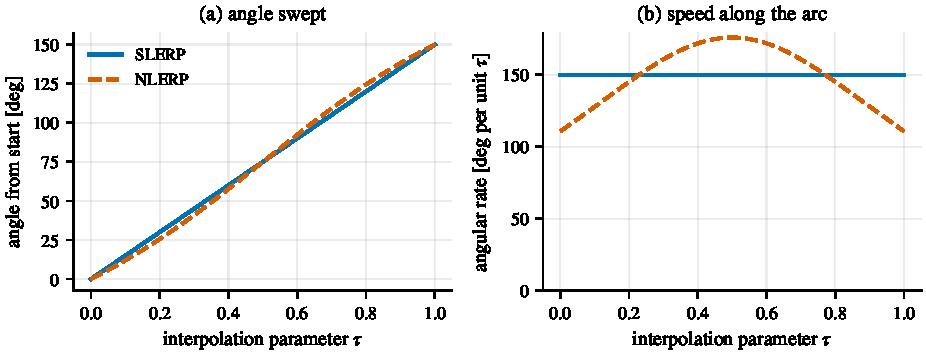
\includegraphics[width=0.84\textwidth]{fig_slerp.pdf}
  \caption{Interpolating between two attitudes $150^\circ$ apart. SLERP sweeps the angle uniformly in the interpolation parameter; normalized linear
  interpolation (NLERP) follows the same path but at a non-uniform speed, fastest in the middle.}
  \label{fig:slerp}
\end{figure}

Ground truth and IMU data rarely share timestamps with images, so attitudes must be interpolated. The correct interpolation follows the
shortest great arc at constant angular velocity: \term{spherical linear interpolation} (SLERP),
\begin{equation}
  q(\tau) = q_0 \qprod \Exp_q\!\big(\tau\,\Log_q(q_0\inv\qprod q_1)\big)
          = \frac{\sin((1 - \tau)\Omega)}{\sin\Omega}\,q_0 + \frac{\sin(\tau\Omega)}{\sin\Omega}\,q_1,
  \qquad \tau\in[0,1],
\end{equation}
with $\cos\Omega = q_0\T q_1$ after flipping the sign of $q_1$ if needed so that $q_0\T q_1 \ge 0$. The first form (using the exponential and
logarithm of \cref{ch:lie}) shows that the relative rotation is applied with a uniformly growing angle; the second is the formula for
interpolating along a great circle of the sphere. Component-wise linear interpolation followed by normalization (NLERP) follows the same
path at a non-uniform speed (\cref{fig:slerp}); it is acceptable only for small angles.

% ==============================================================================
\section{Rigid-body transformations}

A rigid transformation combines a rotation and a translation. Point coordinates transform as
\begin{equation}
  p_w = R_{wb}\,p_b + p_{wb}
  \quad\Longleftrightarrow\quad
  \begin{bmatrix} p_w \\ 1 \end{bmatrix} = \underbrace{\begin{bmatrix} R_{wb} & p_{wb} \\ 0 & 1 \end{bmatrix}}_{T_{wb}}
  \begin{bmatrix} p_b \\ 1 \end{bmatrix}.
\end{equation}
Appending a 1 to the point (\emph{homogeneous coordinates}, developed in \cref{ch:camera}) turns the affine map into a single matrix product.
The $4\times4$ matrices of this form make up the group $\SE$ of rigid motions. Composition and inversion follow from block multiplication:
\begin{equation}
  T_{wc} = T_{wb}T_{bc} = \begin{bmatrix} R_{wb}R_{bc} & R_{wb}p_{bc} + p_{wb} \\ 0 & 1\end{bmatrix},
  \qquad
  T_{wb}\inv = T_{bw} = \begin{bmatrix} R_{wb}\T & -R_{wb}\T p_{wb} \\ 0 & 1 \end{bmatrix}.
  \label{eq:se3-compose}
\end{equation}
The camera pose in the world therefore is $R_{wc} = R_{wb}R_{bc}$ and $p_{wc} = p_{wb} + R_{wb}p_{bc}$, and a world point $p_f$ has camera coordinates
\begin{equation}
  p_c = R_{bc}\T\big(R_{wb}\T(p_f - p_{wb}) - p_{bc}\big),
  \label{eq:world-to-camera}
\end{equation}
which is the first half of the camera measurement model (AGENTS.md C6).

\begin{pitfall}[points versus directions]
Translations apply to points, not to free vectors. A velocity, a gravity vector or a bearing direction transforms with the rotation only,
$v_w = R_{wb}v_b$. In homogeneous coordinates directions carry a $0$ in the fourth component, which drops the translation automatically.
\end{pitfall}

% ==============================================================================
\section{Rotational kinematics}
\label{sec:rot-kinematics}

\subsection{Angular velocity}

Let $R(t) = R_{wb}(t)$ describe a rotating body. Differentiating $R\T R = I$ gives $\dot R\T R + R\T\dot R = 0$, so $R\T\dot R$ is skew-symmetric and
equals $\sx{\omega_b}$ for a unique vector $\omega_b$:
\begin{equation}
  \dot R_{wb} = R_{wb}\,\sx{\omega_b} = \sx{\omega_w}\,R_{wb}, \qquad \omega_w = R_{wb}\,\omega_b ,
  \label{eq:rdot}
\end{equation}
where the second form uses \eqref{eq:skew-rot}. Why is $\omega$ an angular velocity? A point fixed in the body, with constant body coordinates $r_b$,
has world coordinates $r_w = R_{wb}r_b$ and velocity $\dot r_w = \dot R_{wb}r_b = \sx{\omega_w}R_{wb}r_b = \omega_w\times r_w$: every point moves as if the body
were spinning about the axis $\omega_w$ through the origin with angular speed $\|\omega\|$. $\omega_b$ is this angular velocity of $B$ relative to $W$,
expressed in $B$, and it is exactly what a strapdown gyroscope measures (up to bias and noise). The two forms of \eqref{eq:rdot} are the
kinematic origin of the two perturbation conventions of \cref{ch:lie}: a body-frame quantity multiplies on the right, a world-frame quantity on
the left.

\begin{proposition}[Constant body rate]
\label{prop:const-rate}
If $\omega_b$ is constant on $[t_0, t_0 + \Dt]$, then $R(t_0 + \Dt) = R(t_0)\exp(\Dt\sx{\omega_b})$.
\end{proposition}
\begin{proof}
$R(t) = R(t_0)\exp((t - t_0)\sx{\omega_b})$ satisfies \eqref{eq:rdot} by \cref{prop:matexp}, and the solution is unique (\cref{thm:lti-solution}).
\end{proof}

This exact solution is the basis of the multiplicative attitude update used in every integration scheme of \cref{ch:strapdown}. When the
rate varies, the update is still applied step by step with the rate held constant over each short step (\cref{sec:lie-euler}). Note that the
solution is \emph{not} $R(t_0) + \Dt\, R(t_0)\sx{\omega_b}$, which would leave $\SO$.

\subsection{Quaternion kinematics}

The quaternion counterpart of \eqref{eq:rdot} is
\begin{equation}
  \dot q_{wb} = \tfrac12\, q_{wb} \qprod [0,\ \omega_b] = \tfrac12\,\Omega(\omega_b)\,q_{wb},
  \qquad \Omega(\omega) = [\,[0, \omega]\,]_R = \begin{bmatrix} 0 & -\omega\T \\ \omega & -\sx{\omega}\end{bmatrix},
  \label{eq:qdot}
\end{equation}
with constant-rate solution $q(t_0 + \Dt) = q(t_0)\qprod\big[\cos\tfrac{\|\omega\|\Dt}{2},\ \sin\tfrac{\|\omega\|\Dt}{2}\,\tfrac{\omega}{\|\omega\|}\big]$. To derive
\eqref{eq:qdot}, compose $q(t + \dd t) = q(t) \qprod \dd q$, where $\dd q$ is the small body-frame rotation by $\omega_b\,\dd t$. By
\eqref{eq:quat-axis-angle}, $\dd q = [1,\ \tfrac12\omega_b\,\dd t] + O(\dd t^2)$, so $q(t + \dd t) - q(t) = q\qprod[0, \tfrac12\omega_b]\,\dd t$. The factor $\tfrac12$ is
the half angle again.

\subsection{Derivatives in a rotating frame}

Differentiating $v_w = R_{wb}v_b$ with \eqref{eq:rdot} gives the \term{transport theorem}
\begin{equation}
  \dot v_w = R_{wb}\big(\dot v_b + \omega_b \times v_b\big):
  \label{eq:transport}
\end{equation}
the rate of change seen from the fixed frame equals the rate seen in the rotating frame plus the change due to the rotation of the frame itself.
Applying it twice to the position $r$ of a particle relative to a frame rotating with angular velocity $\Omega$ (constant) gives the acceleration
in the fixed (inertial) frame, expressed in rotating coordinates:
\begin{equation}
  a_{\mathrm{inertial}} = \ddot r + 2\,\Omega\times\dot r + \Omega\times(\Omega\times r),
  \label{eq:coriolis}
\end{equation}
where $\ddot r$ and $\dot r$ are the acceleration and velocity seen in the rotating frame. The extra terms are the \term{Coriolis acceleration}
$2\Omega\times\dot r$ and the \term{centripetal acceleration} $\Omega\times(\Omega\times r)$. This formula is the working principle of the vibratory MEMS gyroscope
(\cref{ch:imu}), and it tells us what we neglect by treating the world frame as inertial.

\subsection{The Earth is not an inertial frame}

The world frame $W$ is fixed to the Earth, which rotates at $\Omega_e = 7.292\times10^{-5}$~rad/s. Three effects follow; their sizes justify the
project's simplifications.
\begin{itemize}
  \item \emph{Gyroscopes sense the Earth rate.} $7.3\times10^{-5}$~rad/s is comparable to the bias instability of the EuRoC ADIS16448 and far below its
        noise over short horizons. The project neglects it; its constant body-frame component (while the attitude changes little) is absorbed
        by the gyro bias estimate. High-grade systems model it explicitly and can even find north from it (gyrocompassing).
  \item \emph{Centripetal acceleration.} The term $\Omega_e\times(\Omega_e\times r)$ reaches $0.034~\mathrm{m/s^2}$ at the equator. It is absorbed into the
        local gravity vector: \emph{gravity}, as measured by a plumb line, is gravitation plus this centrifugal term. Its magnitude varies from
        $9.780~\mathrm{m/s^2}$ at the equator to $9.832~\mathrm{m/s^2}$ at the poles; the project uses a constant $9.81$ (AGENTS.md C5), accurate to about
        $10^{-3}$ relative in Zurich, where EuRoC was recorded.
  \item \emph{Coriolis acceleration.} $2\Omega_e\times v$ is about $1.5\times10^{-4}~\mathrm{m/s^2}$ at 1~m/s: below accelerometer noise and bias for a small
        drone, and neglected.
\end{itemize}
Over the minutes and hundreds of meters of a EuRoC sequence, the world frame may therefore be treated as inertial and flat, with constant
gravity.

\begin{takeaways}
\begin{itemize}
  \item $R_{wb}$ maps body coordinates to world coordinates; its columns are the body axes in the world. Adjacent subscripts must match.
  \item Every rotation is an axis-angle rotation, $R = I + \sin\theta\sx{u} + (1-\cos\theta)\sx{u}^2$; $\tr R = 1 + 2\cos\theta$.
  \item Euler angles have intrinsic and extrinsic readings and a singularity at $\pm90^\circ$ pitch; they stay out of the estimator.
  \item Hamilton unit quaternions compose like matrices; $q$ and $-q$ are the same rotation; the quaternion of a rotation by $\theta$ uses $\theta/2$.
  \item Eigen's constructor is $w$-first, its storage $w$-last, EuRoC is $w$-first. JPL formulas must be re-derived, not copied.
  \item $\dot R_{wb} = R_{wb}\sx{\omega_b}$; with constant $\omega_b$ the update $R \leftarrow R\exp(\Dt\sx{\omega_b})$ is exact.
  \item Derivatives in rotating frames pick up $\omega\times$ terms; for a small drone over minutes, the Earth's rotation is negligible.
\end{itemize}
\end{takeaways}

\begin{exercises}
  \item Show that the columns of any $R \in \SO$ are orthonormal and that $\det R = +1$ implies the third column is the cross product of the first two.
  \item Verify $R_x(90^\circ)R_y(90^\circ) \neq R_y(90^\circ)R_x(90^\circ)$ by computing both products, and describe each rotation physically.
  \item Derive \eqref{eq:euler-rates} from \eqref{eq:zyx} and $\sx{\omega_b} = R\T\dot R$.
  \item Convert the rotation of the worked example ($120^\circ$ about $(1,1,1)/\sqrt3$) to ZYX Euler angles.
  \item Prove that $[p]_L[q]_R = [q]_R[p]_L$. What does this say about associativity of the quaternion product?
  \item Show that $R(-q) = R(q)$ and compute the quaternion of a $270^\circ$ rotation about $z$ in its canonical form ($w \ge 0$). What rotation angle and
        axis does the canonical form describe?
  \item Implement Shepperd's method and test it on rotations by $0^\circ$, $90^\circ$, $179.9999^\circ$ and $180^\circ$.
  \item Write a function that converts a EuRoC ground-truth row into $p_{wb}$, $q_{wb}$, $v_{wb}$, $b_g$ and $b_a$. Design a fixture row whose values would
        expose a swapped $w/z$ and swapped biases.
  \item Given $T_{bc}$ from \code{cam0/sensor.yaml} (\cref{app:euroc}), compute the camera's optical axis in body coordinates.
  \item Show that if $\omega_b$ varies in time, $R(t) = R(0)\exp\big(\int_0^t\sx{\omega_b}\,\dd s\big)$ is in general \emph{wrong}. Construct a counterexample with
        piecewise-constant rates.
  \item Derive \eqref{eq:coriolis} by applying \eqref{eq:transport} twice.
\end{exercises}
% Solutions to the exercises of Chapter 7.
\begin{solutions}
  \item Write $R = [r_1\ r_2\ r_3]$. The entry $(i, j)$ of $R\T R = I$ is $r_i\T r_j = \delta_{ij}$: the columns are orthonormal. The unit vectors orthogonal
        to both $r_1$ and $r_2$ are exactly $\pm r_1\times r_2$ (a unit vector, by Lagrange's identity), so $r_3 = \pm r_1\times r_2$. The determinant is the
        triple product $\det R = r_3\T(r_1\times r_2) = \pm\|r_1\times r_2\|^2 = \pm1$, so $\det R = +1$ selects $r_3 = r_1\times r_2$: the body axes form a
        right-handed frame.

  \item From the elementary matrices,
        \[
          R_x(90^\circ)R_y(90^\circ) = \begin{bmatrix}0 & 0 & 1\\ 1 & 0 & 0\\ 0 & 1 & 0\end{bmatrix}, \qquad
          R_y(90^\circ)R_x(90^\circ) = \begin{bmatrix}0 & 1 & 0\\ 0 & 0 & -1\\ -1 & 0 & 0\end{bmatrix}.
        \]
        The first sends $e_x \to e_y$, $e_y \to e_z$, $e_z \to e_x$ (its columns): it cycles the axes, a $120^\circ$ rotation about $(1,1,1)/\sqrt3$. The
        second has trace 0 (angle $120^\circ$) and $(R - R\T)\veeop = (1, 1, -1)$, so it is a $120^\circ$ rotation about $(1, 1, -1)/\sqrt3$. Physically, read
        as intrinsic sequences: the first turns a book $90^\circ$ about its $x$-axis and then $90^\circ$ about its new $y$-axis; the second does the two
        quarter turns in the other order and leaves the book in a different orientation.

  \item Write $R = R_zR_yR_x$ with $\dot R_z = \dot\psi R_z\sx{e_z}$, $\dot R_y = \dot\vartheta R_y\sx{e_y}$, $\dot R_x = \dot\varphi R_x\sx{e_x}$. Then
        \[
          R\T\dot R = \dot\psi\,R_x\T R_y\T\sx{e_z}R_yR_x + \dot\vartheta\,R_x\T\sx{e_y}R_x + \dot\varphi\,\sx{e_x}
          = \big[\dot\psi\,R_x\T R_y\T e_z + \dot\vartheta\,R_x\T e_y + \dot\varphi\,e_x\big]_\times
        \]
        by \eqref{eq:skew-rot}. With $R_y\T e_z = (-s_\vartheta, 0, c_\vartheta)$, $R_x\T(-s_\vartheta, 0, c_\vartheta) = (-s_\vartheta, s_\varphi c_\vartheta, c_\varphi c_\vartheta)$ and
        $R_x\T e_y = (0, c_\varphi, -s_\varphi)$,
        \[
          \omega_b = \begin{bmatrix} 1 & 0 & -s_\vartheta \\ 0 & c_\varphi & s_\varphi c_\vartheta \\ 0 & -s_\varphi & c_\varphi c_\vartheta \end{bmatrix}
                     \begin{bmatrix}\dot\varphi\\ \dot\vartheta\\ \dot\psi\end{bmatrix}.
        \]
        The matrix has determinant $c_\vartheta$. Solving the last two rows gives $\dot\vartheta = c_\varphi\omega_y - s_\varphi\omega_z$ and
        $\dot\psi = (s_\varphi\omega_y + c_\varphi\omega_z)/c_\vartheta$, and the first row gives $\dot\varphi = \omega_x + s_\vartheta\dot\psi$, which is \eqref{eq:euler-rates}.
        The determinant $c_\vartheta$ vanishes at $\vartheta = \pm90^\circ$: gimbal lock.

  \item The rotation is the axis-cycling matrix of Exercise 7.2, $R = \begin{bmatrix}0 & 0 & 1\\ 1 & 0 & 0\\ 0 & 1 & 0\end{bmatrix}$. With the conversion formulas,
        $\vartheta = \atantwo(-R_{31}, \sqrt{R_{11}^2 + R_{21}^2}) = \atantwo(0, 1) = 0$, $\varphi = \atantwo(R_{32}, R_{33}) = \atantwo(1, 0) = 90^\circ$ and
        $\psi = \atantwo(R_{21}, R_{11}) = \atantwo(1, 0) = 90^\circ$: yaw $90^\circ$, pitch $0$, roll $90^\circ$. Check: $R_z(90^\circ)R_x(90^\circ)$ reproduces $R$, as the worked
        example $q_z\qprod q_x$ already showed.

  \item Apply both sides to an arbitrary quaternion $r$. By definition $[q]_Rr = r\qprod q$ and $[p]_Lr = p\qprod r$, so
        \[
          [p]_L[q]_R\,r = p\qprod(r\qprod q), \qquad [q]_R[p]_L\,r = (p\qprod r)\qprod q .
        \]
        The two agree for every $r$ exactly because the Hamilton product is associative, so the matrices are equal. (Multiplying out the blocks and
        using $\sx{a}\sx{b} = ba\T - (a\T b)I$ confirms it directly.) Conversely, the identity $[p]_L[q]_R = [q]_R[p]_L$ for all $p, q$ \emph{is} the
        statement of associativity: multiplying on the left and on the right are commuting operations.

  \item $R(q)$ in \eqref{eq:quat-to-rot} is a homogeneous quadratic in the components of $q$, so $R(-q) = (-1)^2R(q) = R(q)$. A $270^\circ$ rotation about
        $z$ has
        \[
          q = \big[\cos135^\circ,\ \sin135^\circ e_z\big] = \big[-\tfrac{\sqrt2}{2},\ (0, 0, \tfrac{\sqrt2}{2})\big].
        \]
        Its scalar part is negative, so the canonical form is $-q = [\tfrac{\sqrt2}{2},\ (0, 0, -\tfrac{\sqrt2}{2})]$. It describes a rotation by
        $2\arccos(\tfrac{\sqrt2}2) = 90^\circ$ about $-e_z$: the same rotation as $270^\circ$ about $+e_z$, reached the short way round. Canonicalization
        always yields an angle in $[0, \pi]$.

  \item A direct implementation picks the largest of the four squared components, computed from the diagonal:
\begin{lstlisting}[style=py]
def shepperd(R):
    t = np.trace(R)
    c = [1 + t, 1 + R[0,0] - R[1,1] - R[2,2], 1 - R[0,0] + R[1,1] - R[2,2], 1 - R[0,0] - R[1,1] + R[2,2]]
    i = int(np.argmax(c)); s = 2 * np.sqrt(c[i])          # s = 4 * (largest component)
    a, b, d = R[2,1] - R[1,2], R[0,2] - R[2,0], R[1,0] - R[0,1]   # 4wx, 4wy, 4wz
    e, f, g = R[0,1] + R[1,0], R[0,2] + R[2,0], R[1,2] + R[2,1]   # 4xy, 4xz, 4yz
    q = [[s/4, a/s, b/s, d/s], [a/s, s/4, e/s, f/s], [b/s, e/s, s/4, g/s], [d/s, f/s, g/s, s/4]][i]
    return np.array(q) if q[0] >= 0 else -np.array(q)
\end{lstlisting}
        Testing against the quaternion used to build each matrix (axis $(1, -2, 0.5)/\|\cdot\|$) gives errors of $0$, $3\times10^{-16}$, $2\times10^{-18}$ and
        $10^{-16}$ at $0^\circ$, $90^\circ$, $179.9999^\circ$ and $180^\circ$. The naive formula $w = \tfrac12\sqrt{1 + \tr R}$, $v = (R - R\T)\veeop/4w$ is exact at the first two,
        wrong by $9\times10^{-6}$ at $179.9999^\circ$ (it divides by $w \approx 9\times10^{-7}$, computed from the difference $1 + \tr R \approx 3\times10^{-12}$), and
        undefined at $180^\circ$.

  \item The ground-truth row is \code{timestamp, p\_x, p\_y, p\_z, q\_w, q\_x, q\_y, q\_z, v\_x, v\_y, v\_z, bw\_x, bw\_y, bw\_z, ba\_x, ba\_y, ba\_z} (AGENTS.md C7).
        In C++ the parser constructs each piece explicitly:
\begin{lstlisting}
p_wb = Eigen::Vector3d(r[1], r[2], r[3]);
q_wb = Eigen::Quaterniond(r[4], r[5], r[6], r[7]).normalized();  // w first
v_wb = Eigen::Vector3d(r[8], r[9], r[10]);
b_g  = Eigen::Vector3d(r[11], r[12], r[13]);   // gyro bias comes first
b_a  = Eigen::Vector3d(r[14], r[15], r[16]);
\end{lstlisting}
        A good fixture row makes every plausible mistake produce a detectably different result: all quaternion components distinct and of
        different signs, e.g.\ $q = (w, x, y, z) = (0.8, 0.2, -0.4, 0.4)$ (unit norm), so that reading it as $[x, y, z, w]$ gives a different rotation;
        biases of different magnitudes and signs, e.g.\ $b_g = (0.01, 0.02, 0.03)$ and $b_a = (-0.1, -0.2, -0.3)$, so that swapping them is visible;
        and position and velocity that differ in every component. The test asserts each field and also checks that $R(q)\,e_x$ equals the column
        computed by hand, which catches a wrong constructor order even when the norm is unchanged. A row with the identity quaternion, or with
        equal biases, would let all these bugs pass.

  \item The optical axis is the camera's $z$-axis; in body coordinates it is $R_{bc}e_z$, the third column of the rotation block of $T_{bc}$. With the
        values of \cref{app:euroc} it is $(0.0041, 0.0257, 0.9997)$: the camera looks along the body $+z$-axis, tilted by $\arccos(0.9997) = 1.5^\circ$. The
        other columns show the camera $x$-axis along body $+y$ and the camera $y$-axis along body $-x$; since the EuRoC IMU's $x$-axis points up at
        rest, the image $y$-axis (rows, increasing downwards) indeed points down.

  \item By \cref{prop:stm} the formula holds only if the matrices $\sx{\omega_b(t)}$ commute for all $t$, i.e.\ if $\omega_b(t)$ keeps a fixed direction. Counterexample:
        $\omega_b = (\pi/2, 0, 0)$ on $[0, 1)$ and $(0, \pi/2, 0)$ on $[1, 2)$. By \cref{prop:const-rate} applied to each segment the true attitude is
        $R(2) = R(0)R_x(90^\circ)R_y(90^\circ)$, a $120^\circ$ rotation relative to $R(0)$ (Exercise 7.2). The formula gives
        $R(0)\exp(\sx{(\pi/2, \pi/2, 0)})$, a $127^\circ$ rotation about $(1, 1, 0)/\sqrt2$, which is wrong by $1.1$~rad. This is the coning error in its
        crudest form (\cref{sec:coning}).

  \item Let $r_I = Rr$ be the particle's position in inertial coordinates, with $\dot R = R\sx{\Omega}$ and $\Omega$ constant. The transport theorem gives
        $\dot r_I = R(\dot r + \Omega\times r) = Ru$ with $u = \dot r + \Omega\times r$. Applying it again to $u$,
        \[
          \ddot r_I = R(\dot u + \Omega\times u) = R\big(\ddot r + \Omega\times\dot r + \Omega\times\dot r + \Omega\times(\Omega\times r)\big),
        \]
        using $\dot\Omega = 0$. Expressed in rotating coordinates ($R\T\ddot r_I$), the inertial acceleration is
        $\ddot r + 2\,\Omega\times\dot r + \Omega\times(\Omega\times r)$, which is \eqref{eq:coriolis}. The factor 2 comes from the two applications, each contributing
        one $\Omega\times\dot r$.
\end{solutions}

